\chapter{Statistics}\label{chapter:stats}

This appendix provides a refresher in some of the statistics
underlying machine learning and natural language processing.




\section{Discrete Probability Distributions}

\subsection{Bernoulli Distribution}

The Bernoulli distribution has binary outcomes 0 and 1, with outcome 1
conventionally referred to as ``success.''  The distribution has a
single parameter $\theta \in [0,1]$ for the chance of success.  If a
random variable $X$ has a Bernoulli distribution with parameter
$\theta$ we write $X \sim \dbern{\theta}$.  The resulting probablity
distribution for $x \sim \dbern{\theta}$ is defined for $x \in
\setext{0,1}$ by
%
\begin{equation}
p_X(x) = \theta^{x} \times (1 - \theta)^{1-x}.
\end{equation}
%
Working out the cases, if $x=1$, we have $p_X(x) = \theta$ and
if $x=0$, we have $p_X(x) = 1 - \theta$.

The variance and standard deviation for $X \sim \dbern{\theta}$ are
given by
%
\begin{equation}
\var{X} = \theta (1-\theta)
\ \ \ \ \ \mbox{and} \ \ \ \ \
\sd{X} = \sqrt{\theta (1 - \theta)}.
\end{equation}


\subsection{Binomial Distribution}\label{section:stats-binomial-distribution}

The binomial distribution is parameterized by a chance-of-success
parameter $\theta \in [0,1]$ and a number-of-trials parameter $N \in
\nats$.  If a random variable $X$ has a binomial distribution with
parameters $\theta$ and $N$, we write $X \sim \dbin{\theta}{N}$.  The
resulting probability distribution is defined for $n \in 0{:}N$ by
%
\begin{equation}
p_X(n) = {N \choose n} \ \theta^{n} \ (1-\theta)^{N-n}.
\end{equation}
%
%

The variance and standard deviation of a binomially-distributed random
variable $X \sim \dbin{\theta}{N}$ are given by
%
\begin{equation}
\hfill
\var{X} = \frac{\theta (1 - \theta)}{N} 
\hspace*{0.25in}
\mbox{and}
\hspace*{0.25in}
\sd{X} = \sqrt{\frac{\theta (1 - \theta)}{N}}.
\hfill
\end{equation}
%

We are often more interested in the percentage of the $N$ trials that
resulted in success, which is given by the random variable $X/N$ (note
that $N$ is a constant here).  The variable $X/N$ is scaled to be
between 0 and 1.  With large $N$, $X/N$, will be approximately equal
to $\theta$ for almost every trial.  The variance and standard
deviation of $X/N$ are derived in the usual way, by dividing by the
constant $N$,
%
\begin{equation}
\var{X/N} = \theta (1 - \theta) 
\hspace*{0.25in}
\mbox{and}
\hspace*{0.25in}
\sd{X/N} = \sqrt{\theta (1-\theta)}.
\end{equation}


\subsection{Discrete Distribution}

The discrete distribution generalizes the Bernoulli distribution to
$K$ outcomes.  A discrete distribution is parameterized by a vector
$\theta \in [0,1]^K$ such that
%
\begin{equation}
\sum_{k=1}^K \theta_k = 1.
\end{equation}

If the variable $X$ has a discrete distribution with parameter
$\theta$, we write $X \sim \ddisc{\theta}$.  The resulting probabilty
distribution for $X \sim \ddisc{\theta}$ is defined for $x \in 1{:}K$
by
%
\begin{equation}
p_X(x) = \theta_x.
\end{equation}
%

If $K=2$, a discrete distribution has the same distribution
over outcomes 1 and 2 as a Bernoulli has over outcomes 0 and 1.  
In symbols, for $x \in \setext{0,1}$, we have
%
\begin{equation}
\dbern{x|\theta} = \ddisc{x+1|\vecext{1-\theta,\theta}}
\end{equation}

Note that if we collapse categories together so that we
are left with two outcomes (either one versus all, or
one subset versus another subset), we are left with
a Bernoulli distribution.


\subsection{Multinomial Distribution}

Multinomials generalize discrete distributions to counts in the same
way that binomials generalize Bernoulli distributions.  Given a
$K$-dimensional discrete parameter $\theta$ and a number of trials
$N$, the multinomial distribution assigns probabilities to
$K$-dimesnional vectors of counts (non-negative integers in $\nats$)
that sum to $N$.  If a vector random variable $X$ is distributed as a
multinomial with discrete parameter $\theta$ and number of trials $N$,
we write $X \sim \dmulti{\theta,N}$.  For a variable $X \sim
\dmulti{\theta,N}$, the probability assigned to outcome $x \in
\nats^K$ where $\sum_{k=1}^K x_k = N$, is
%
\begin{equation}
p_X(x) = {N \choose {x_1,\ldots,x_K}} \prod_{k=1}^K \theta_k^{x_k}.
\end{equation}
%
where we the normalizing term is a multinomial coefficient as defined
in \refsec{maths-multinomial-coefficient}.






\section{Continuous Probability Distributions}

\subsection{Normal Distribution}\label{section:stats-normal-distribution}



\subsection{$\chi^2$ Distribution}\label{section:stats-chi-squared-distribution}

The $\chi^2$ distribution with $n$ degrees of freedom arises as the
sum of the squares of $n$ independent unit normal distributions (see
\refsec{stats-normal-distribution}).  In symbols, if $X_n \sim \dnorm(0,1)$
for $n \in 1{:}N$, then 
%
\begin{equation}
Y = \sum_{n=1}^N X_n^2
\end{equation}
%
has a $\chi^2$ distribution with $N$ degrees of freedom.

If a variable $X$ has a $\chi^2$ distribution with $N$ degrees of
freedom, we write $X \sim \dchisq{N}$.  The probability distribution
for $X$ is defined for $x \in [0,\infty)$ by
%
\begin{equation}
p_X(x) = \frac{1}{2^{N/2} \ \Gamma(n/2)} \ x^{N/2-1} \ \exp(-x/2).
\end{equation}
%

If $X \sim \dchisq{N}$, then the mean, variance and standard deviation of $X$ are
%
\begin{equation}
\expect{X} = N,
\ \ \ \ \ 
\var{X} = 2n, \mbox{ and}
\ \ \ \ \  
\sd{X} = \sqrt{2n}.
\end{equation}


\section{Information Theory}\label{section:stats-information-theory}

Information theory was originally developed by Claude Shannon to model
the transmission of messages over noisy channels such as telephones
or telegraphs.%
%
\footnote{Claude Shannon. 1948.  A mathematical theory of
  communication.  {\it Bell System Technical Journal} {\bf
    27}:379--423 and {\bf 27}:623--656.}

\subsection{Entropy}\label{section:stats-entropy}

Entropy is an information-theoretic measure of the randomness of a
distribution.  


The entropy of a random variable $X$ is most easily expressed as the
expectation of the negative log probability of the variable,
%
\begin{equation}
\entropy{X} = \expect{- \log_2 p_X(X)}.
\end{equation}
%
Because we use base 2, the results are in units of binary digits,
otherwise known as bits.

For a discrete random variable $X$, unfolding the expectation notation
yields
%
\begin{equation}
\entropy{X} = - \sum_{n \in \nats} p_X(n) \ \log_2 p_X(n).
\end{equation}
%
For a continous random variable $X$, we replace the summations
over natural numbers with integration over the real numbers,
%
\begin{equation}
\entropy{X} = - \int_{-\infty}^{\infty} p_X(x) \ \log_2 p_X(x) \ dx
\end{equation}

For example, if we have a Bernoulli-distributed random
variable $Y \sim \dbern{\theta}$, its entropy is
%
\begin{align}
\entropy{Y} &= - p_Y(1) \log_2 p_Y(1) - p_Y(0) \log_2 p_Y(0)
\\
&= - \theta \log_2 \theta - (1 - \theta) \log_2 (1 - \theta).
\end{align}
%
A plot of $\entropy{Y}$ for $Y \sim \dbern{\theta}$ is provided
in \reffig{bern-entropy}.
%
\begin{figure}
\begin{center}
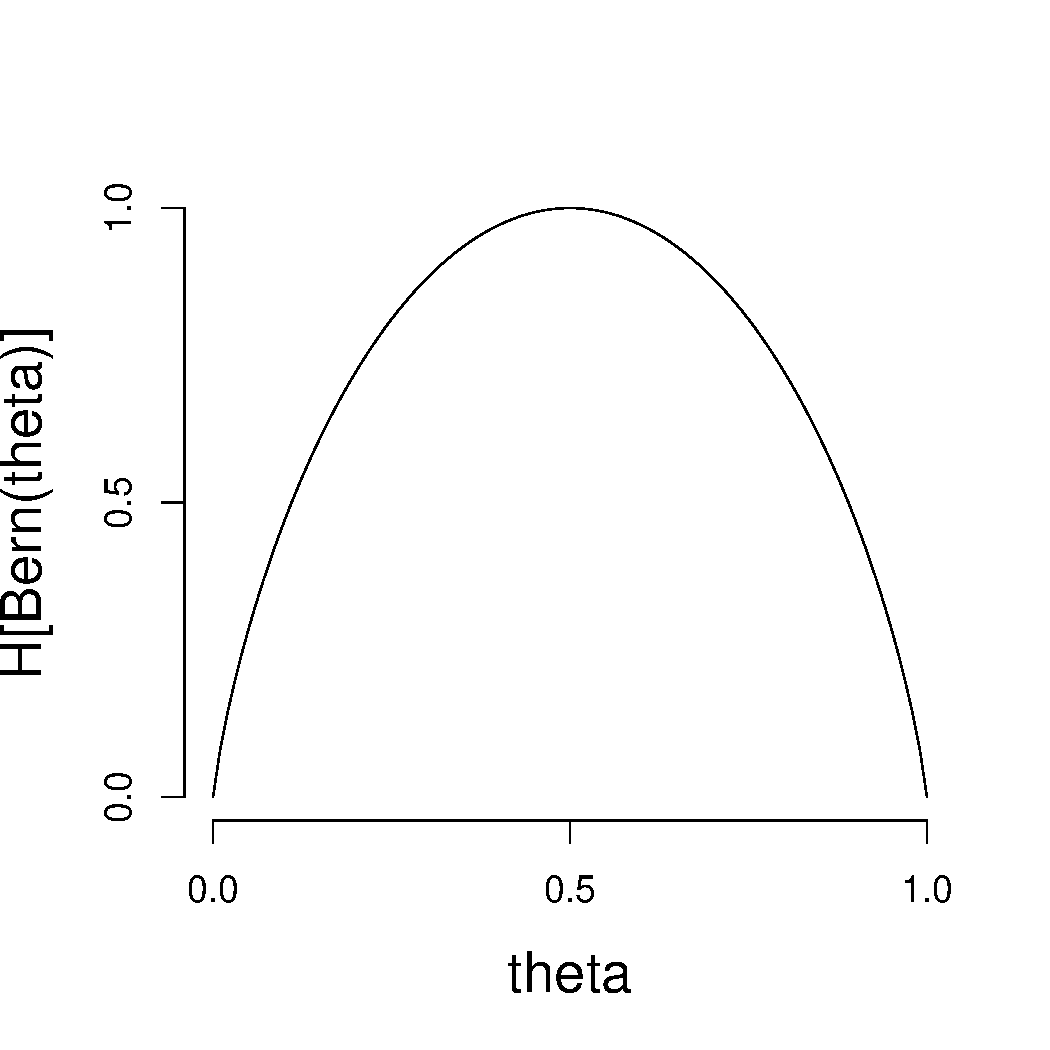
\includegraphics[height=1.75in]{pdfs/bern-entropy.pdf}
\end{center}%
\vspace*{-18pt}
\caption{Entropy of a random variable distributed as $\dbern{\theta}$.}\label{fig:bern-entropy}
\end{figure}
%
The graph makes it clear that when $\theta=0$ or $\theta=1$, the
outcome is certain, and therefore the entropy is 0.  The maximum
entropy possible for a Bernoulli distribution is 1 bit, achieved at
$\theta = 0.5$.  


\subsubsection{Entropy and Compression}

Entropy has a natural interpretation in terms of compression.  Suppose
we want to send the a message $X$ which might take on values in
$\nats$.%
%
\footnote{We can always code sequences of characters as numbers, as
originally noted by Kurt G\"odel, and as explained in any introductory
computer science theory text.  Just think of a string as representing
a number in the base of the number characters.}
%
If the sender and receiver both know the distribution $p_X$
of outcomes, the expected cost to send the message is $\entropy{X}$
bits.  For instance, if we need to send a bit with value 0 or 1, and
each outcome is equally likely, it will require 1 bit to send the
message.  On the other hand, if one outcome is more likely than the
other, we can save space (if we have repeated messages to send;
otherwise, we must round up).


\subsection{Joint Entropy}\label{section:stats-joint-entropy}

We can measure the entropy of two variables $X$ and $Y$ by measuring
the entropy of their joint distribution $p_{X,Y}$, generalizing our
definition to
%
\begin{equation}
\entropy{X,Y} = \expect{\log_2 p_{X,Y}(x,y)}.
\end{equation}
%
For instance, with discrete $X$ and $Y$, this works out to
%
\begin{equation}
\entropy{X,Y} = - \sum_{x} \sum_{y} p_{X,Y}(x,y) \ \log_2 p_{X,Y}(x,y).
\end{equation}
%

Joint entropy is symmetric, so that
%
\begin{equation}
\entropy{X,Y} = \entropy{Y,X}.
\end{equation}

\subsection{Conditional Entropy}\label{section:stats-conditional-entropy}

We can measure the entropy of a variable $X$ conditional on knowing
the value of another variable $Y$.  The expectation-based definition
is thus 
%
\begin{equation}
\condentropy{X}{Y} = \expect{-\log_2 p_{X|Y}(X|Y)}.
\end{equation}
%
In the case of discrete $X$ and $Y$, this works out to
%
\begin{align}
\condentropy{X}{Y} 
&= - \sum_y \sum_x p_{X,Y}(x,y) \ \log_2 p_{X|Y}(x|y)
\\
&= - \sum_y p_Y(y) \sum_x p_{X|Y}(x|y) \ \log_2 p_{X|Y}(x|y).
\end{align}
%

Conditional entropy, joint entropy and entropy are related as for
probabilty distributions, with
%
\begin{equation}
\entropy{X,Y} = \condentropy{X}{Y} + \entropy{Y}.
\end{equation}


\subsection{Mutual Information}\label{section:stats-mutual-information}

The mutual information between a pair of variables $X$ and $Y$ measures how
much more information there is in knowing their joint distribution than their
individual distributions for prediction.  Using expectations, mutual information
between variables $X$ and $Y$ is defined to be
%
\begin{align}
\mutualinfo{X}{Y} 
&= \expect{-\log_2 \frac{p_{X,Y}(x,y)}{p_X(x) \ p_Y(y)}}
\\
&= \expect{-\log_2 p_{X,Y}(x,y)} + \expect{\log_2 p_X(x)} + \expect{\log_2 p_Y(y)}
\end{align}
%
Another way of looking at mutual information is in terms of
the ratio of a conditional and marginal distribution.  If
we unfold the joint distribution $p_{X,Y}(x,y)$ into the product
of the marginal $p_X(x)$ and conditional $p_Y(y|x)$, we get
%
\begin{equation}
\mutualinfo{X}{Y} 
= \expect{-\log_2 \frac{p_{X|Y}(x|y)}{p_X(x)}}
= \expect{-\log_2 \frac{p_{Y|X}(y|x))}{p_Y(y)}}.
\end{equation}



In the discrete case, this unfolds to
%
\begin{equation}
\mutualinfo{X}{Y} = - \sum_{x,y} p_{X,Y}(x,y) \ \log_2 \frac{p_{X,Y}(x,y)}{p_X(x) \ p_Y(y)}.
\end{equation}
%


Mutual information is symmetric, so that
%
\begin{equation}
\mutualinfo{X}{Y} = \mutualinfo{Y}{X}.
\end{equation}
%
It's related to conditional and joint entropies by the unfolding
in the second step of the definition through
%
\begin{align}
\mutualinfo{X}{Y} &= \entropy{X} + \entropy{Y} - \entropy{X,Y}
\\
&= \entropy{X} - \condentropy{X}{Y}.
\end{align}
%

\subsection{Cross Entropy}\label{section:stats-cross-entropy}

Cross-entropy measures the number of bits required, on average, to
transmit a value of $X$ using the distribution of $Y$ for coding.
Using expectation notation, the definition reduces to
%
\begin{equation}
\xentropy{X}{Y} = \expect{-\log_2 p_Y(X)}.
\end{equation}

In the case of discrete random variables $X$ and $Y$, this works out to
%
\begin{equation}
\xentropy{X}{Y} = - \sum_n p_X(n) \ \log_2 p_Y(n).
\end{equation}
%



\subsection{Divergence}\label{section:stats-divergence}

Kullback-Leibler (KL) divergence is the standard method to compare two
distributions.  Pairs of distributions that have similar probabilities
will have low divergence from each other.  Because KL divergence is
not symmetric, we also consider two standard symmetric variants.

Following the standard convention, our previous infomration
definitions were all in terms of random variables $X$ and $Y$, even
though the definitions only dependeded on their corresponding
probability distributions $p_X$ and $p_Y$.  Divergence is
conventionally defined directly on distributions, mainly to avoid the
case of comparing two different random variables $X$ and $Y$ with the
same distribution $p_X = p_Y$.

\subsubsection{KL Divergence}

Given two discrete distributions $p_X$ and $p_Y$, the KL divergence of
$p_Y$ from $p_X$ is given by
%
\begin{equation}
\kld{p_X}{p_Y}
= \sum_{n=1}^N p_X(n) \log_2 \frac{p_X(n)}{p_Y(n)}.
\end{equation}
%
If there is an outcome $n$ where $p_Y(n) = 0$ and $p_X(n) > 0$, the
divergence is infinite.  We may allow $p_X(n) = 0$ by interpreting $0
\log_2 \frac{0}{p_Y(n)} = 0$ by convention (even if $p_Y(n) > 0$).

If we assume $p_X$ and $p_Y$ arose from random variables $X$ and $Y$,
KL divergence may expressed using expectations as
%
\begin{align}
\kld{p_X}{p_Y} 
&= \expect{\log_2 \frac{p_X(X)}{p_Y(X)}}
\\
&= \expect{\log_2 p_X(X)} - \expect{\log_2 p_Y(X)}
\\
&= \expect{-\log_2 p_Y(X)} - \expect{-\log_2 p_X(X)}
\\
&= \xentropy{X}{Y} - \entropy{X}.
\end{align}
%
This definition makes clear that KL divergence may be viewed as as the
expected penalty in bits for using $p_Y$ to transmit values drawn from
$X$ rather than $p_X$ itself.  In other words, KL divergence is just
the cross-entropy minus the entropy.

Although we do not provide a proof, we note that $\kld{p_X}{p_Y} \geq 0$
for all distributions $p_X$ and $p_Y$.  We further note without proof
that $\kld{p_X}{p_Y} = 0$ if and only if $p_X = p_Y$.


\subsubsection{Symmetrized KL Divergence}\label{section:stats-symmetrized-kl-divergence}

KL divergence is not symmetric in the sense that there exist pairs of
random variables $X$ and $Y$ such that $\kld{p_X}{p_Y} \neq \kld{p_Y}{p_X}$.

There are several divergence measures derived from KL divergence that
are symmetric.  The simplest approach is just to introduce symmetry by
brute force.  The symmetrized KL-divergence $\skld{p_X}{p_Y}$ between
distributions $p_X$ and $p_Y$ is defined by averaging the divergence
of $p_X$ from $p_Y$ and the divergence of $p_Y$ from $p_X$, yielding
gives us
%
\begin{equation}
\skld{p_X}{p_Y} = \frac{1}{2}(\kld{p_X}{p_Y} + \kld{p_Y}{p_X}).
\end{equation}
%
Obviously, $\skld{p_X}{p_Y} = \skld{p_Y}{p_X}$ by definition, so the
measure is symmetric.  As with KL divergence, symmetrized KL
divergence so that, in general, $\skld{p_X}{p_Y} \geq 0$ with
$\skld{p_X}{p_Y} = 0$ if and only if $p_X = p_Y$.

\subsubsection{Jensen-Shannon Divergence}

Another widely used symmetric divergence measure derived from KL divergence
is the Jensen-Shannon divergence.  To compare $X$ and $Y$ using Jensen-Shannon
divergence, we first define a new distribution $p_{Z}$ by averaging
the distributions $p_X$ and $p_Y$, by
%
\begin{equation}\label{eq:jensen-shannon-averge-distro}
p_Z(n) = \frac{1}{2}(p_X(n) + p_Y(n)).
\end{equation}
%
If $X$ and $Y$ are random variables and $Z$ is defined to be
$(X+Y)/2$, then $p_X$, $p_Y$ and $p_Z$ satisfy the above definition.

Given the average distribution $p_Z$, we can define Jensen-Shannon
divergence by taking average divergence of $p_X$ and $p_Y$ from $p_Z$
as defined in \refeq{jensen-shannon-averge-distro}, setting
%
\begin{equation}
\jsd{p_X}{p_Y} = \frac{1}{2}(\kld{p_X}{p_Z} + \kld{p_Y}{p_Z}).
\end{equation}
%
As with the symmetrized KL divergence, Jensen-Shannon divergence is
symmetric by definition.


\subsubsection{LingPipe KL-Divergence Utilities}

KL-divergence is implemented as a static utility method in the
\code{Statistics} utility class in package \code{com.aliasi.stats}.
The method takes two double arrays representing probability
distributions and measures how much the first is like the second.

In order to give you a sense of KL-divergence, we implement a simple
utility in the demo class \code{KlDivergence} to let you try various
values.  The code just parses out double arrays from teh command line
and sends them to the KL function.
%
\codeblock{KlDivergence.1}

The ant target \code{kl} runs the command with the first two arguments
given by properties \code{p.x} and \code{p.y}.  To calculate the example
from above, we have
%
\commandlinefollow{ant -Dp.x="0.2 0.8" -Dp.y="0.4 0.6" kl}
\begin{verbatim}
pX=(0.2, 0.8)     pY=(0.4, 0.6)     
kld=0.13202999942307514    
skld=0.1415037499278844   
jsd=0.03485155455967723
\end{verbatim}
%
The Jensen-Shannon divergence is less than the symmetrized KL
divergence because the interpolated distribution $p_Z$ is closer to
both of the original distributions $p_X$ and $p_Y$ than they are to
each other.

